\documentclass[11pt]{amsart}
\usepackage{amsmath,amssymb,amsthm}
\usepackage{graphicx}
\usepackage[colorlinks=true,linkcolor=blue,citecolor=blue,urlcolor=blue]{hyperref}

\theoremstyle{plain}
\newtheorem{theorem}{Theorem}[section]
\newtheorem{lemma}[theorem]{Lemma}
\newtheorem{proposition}[theorem]{Proposition}
\newtheorem{corollary}[theorem]{Corollary}
\theoremstyle{definition}
\newtheorem{definition}[theorem]{Definition}
\theoremstyle{remark}
\newtheorem{remark}[theorem]{Remark}

\title{The Arithmetic of Time}
\author{Stephanie Alexander}
\email{salexander442@gmail.com}
\date{\today}

\begin{document}


\begin{abstract}
We present a small, self-contained mathematical model of time, formalized in Lean 4 against Mathlib v4.31.0 in the public repository \texttt{github.com/stalex444/arithmetic-of-time}. The model is built from two polynomials: $x^3 - x - 1$, whose real root $\rho \approx 1.324718$ is the plastic number, and $x^4 - x - 1$, whose real root is $Q \approx 1.220744$. Four groups of kernel-verified theorems are proved. (1) Settling: the non-real roots $z$ of $x^3 - x - 1$ contract at the exact rate $\rho \lVert z \rVert^2 = 1$, and on the ring $\mathbb{Z}[\rho]$ this sharpens to a Meyer-type separation inequality $\lvert \sigma_1(x) \rvert \cdot \lVert \sigma_2(x) \rVert^2 \ge 1$ for every nonzero $x$ (\texttt{Time.meyer\_separation}). (2) A boundary dichotomy: every non-real root of the cubic lies strictly inside the unit circle and every non-real root of the quartic strictly outside (\texttt{Time.pisot\_boundary\_dichotomy}), each by a single elementary Vieta reduction; thus $\rho$ is a Pisot number and $Q$ is not. (3) The mechanical word $m(n) = \lfloor (n+1)\beta \rfloor - \lfloor n\beta \rfloor$ of an irrational slope $\beta \in (0,1)$ is two-valued, of density $\beta$, aperiodic, and balanced (\texttt{Time.balanced}). (4) An untunable chain: the constants $\kappa = (Q/\rho)^2$, $r_{\mathrm{in}} = \sqrt{3}/2$, $\chi = Q/\rho$, and $A^* = \sqrt{2\rho} - \sqrt{3/4 - \rho^{-2}}$ satisfy the strict chain $\kappa < r_{\mathrm{in}} < \chi < A^*$ (\texttt{Time.chain\_strict}); the two thresholds are provably not algebraic integers while every monomial $\rho^a Q^b$ is an algebraic unit, so no such monomial can equal a threshold at any integer exponents. Every theorem depends only on the axioms \texttt{propext}, \texttt{Classical.choice}, and \texttt{Quot.sound}, with no \texttt{sorry} and no \texttt{native\_decide}. A numerical companion computes the quasicrystalline diffraction of the mechanical word; the underlying pure-point theorem is cited, not formalized. The paper is a theorem-level study of a mathematical model; no empirical claim about physical time is made.
\end{abstract}
\maketitle

\section{Introduction}\label{sec:intro}

Consider four structural demands one might place on a mathematical carrier of time.
\begin{enumerate}
\item[(i)] \emph{Individuation}: states settle onto a discrete record, and distinct states are never confused.
\item[(ii)] \emph{Irreversibility}: each step is an exact one-way contraction, never undone.
\item[(iii)] \emph{Aperiodicity}: the process never repeats.
\item[(iv)] \emph{Non-randomness}: the succession of steps is maximally even rather than stochastic.
\end{enumerate}
This paper exhibits a concrete arithmetic structure meeting all four demands, with every claim machine-checked or explicitly labeled as cited or computed. One convention is fixed here, once: the word \emph{time} and its cognates in this paper (\emph{moment}, \emph{tick}, \emph{arrow}) are names for the mathematical objects defined below, and carry no content beyond those definitions.

The structure is built from two polynomials: $x^3 - x - 1$, whose real root $\rho \approx 1.324718$ is the plastic number \cite{aarts2001} and, by a classical theorem of Siegel \cite{siegel1944}, the smallest Pisot number; and $x^4 - x - 1$, whose real root is $Q \approx 1.220744$. All results are formalized in Lean 4 against Mathlib v4.31.0 in the public repository \texttt{github.com/stalex444/arithmetic-of-time}; throughout, \emph{kernel-verified} means proved there and checked by the Lean kernel, \emph{classical} or \emph{cited} means a literature theorem not formalized here, and \emph{computed} means numerical evidence from the repository's \texttt{diffraction/} folder. The results fall into four groups.

\emph{Settling and Meyer separation} (demands (i) and (ii)). For the non-real roots $z$ of $x^3 - x - 1$, the transverse dynamics contracts at an \emph{exact} rate: $\rho \lVert z \rVert^2 = 1$, so $\lVert z \rVert = \rho^{-1/2}$ --- one irreversible step (\texttt{Time.tick\_contraction}, \texttt{Time.norm\_z\_eq\_rpow}). On the ring of integers $\mathbb{Z}[\rho]$ this sharpens to a Meyer-type separation inequality: writing $\sigma_1$ for the real and $\sigma_2$ for the complex embedding of $\mathbb{Q}(\rho)$, every nonzero $x \in \mathbb{Z}[\rho]$ satisfies $\lvert \sigma_1(x) \rvert \cdot \lVert \sigma_2(x) \rVert^2 \ge 1$ (\texttt{Time.meyer\_separation}, \texttt{Time.meyer\_separation\_rpow}). Distinct arithmetic states can never be confused within a bounded window, and the contraction is never undone. The same theorems are re-proved by an independent second formalization (\texttt{TimeReplica.meyer\_separation}, \texttt{TimeReplica.certification\_soundness}).

\emph{The Pisot boundary: the cubic settles, the quartic spirals.} Directly from the two defining polynomials, every non-real root $z$ of $x^3 - x - 1$ satisfies $\lVert z \rVert < 1$ (\texttt{Time.cubic\_conj\_norm\_lt\_one}), while every non-real root $w$ of $x^4 - x - 1$ satisfies $\lVert w \rVert > 1$ (\texttt{Time.quartic\_conj\_norm\_gt\_one}); together, $\lVert z \rVert < 1 \wedge 1 < \lVert w \rVert$ (\texttt{Time.pisot\_boundary\_dichotomy}). So $\rho$ is a Pisot number and $Q$ is not \cite{bertin1992}. The proof is elementary and self-contained: writing $\sigma = w + \overline{w}$ and $s = w \overline{w} = \lVert w \rVert^2$ and reducing modulo the Vieta quadratic $w^2 = \sigma w - s$ yields one real identity per polynomial --- $s^3 + s^2 = 1$ for the cubic, forcing $s < 1$, and $s^2 - \sigma^2 s = 1$ for the quartic, forcing $s > 1$ --- one flipped inequality, driven purely by the degree. We are explicit about the tier boundary: this is the concrete settle/spiral dichotomy for these two polynomials; Siegel's theorem that $\rho$ is the \emph{smallest} Pisot number remains classical \cite{siegel1944}, as the required Pisot theory lies outside Mathlib.

\emph{The tick: aperiodic but not random} (demands (iii) and (iv)). For irrational $\beta \in (0,1)$, the mechanical word $m(n) = \lfloor (n+1)\beta \rfloor - \lfloor n\beta \rfloor$ --- a Sturmian object in the tradition of Morse and Hedlund \cite{morsehedlund1940,lothaire2002} --- is kernel-verified to be \emph{two-valued} (\texttt{Time.m\_mem}), of \emph{density} equal to the slope (\texttt{Time.density\_tendsto}, via the exact telescoping identity \texttt{Time.sum\_m\_eq}), \emph{aperiodic} (\texttt{Time.aperiodic}), and \emph{balanced}: the 1-counts of any two windows of equal length differ by at most one (\texttt{Time.balanced}). Balance is the precise ``maximally even, not random'' property of a Sturmian word. The irrationality of the slope, which lies beyond Mathlib, is carried as an explicit hypothesis throughout, never assumed as an axiom.

\emph{The untunable constant chain.} The four algebraic constants $\kappa = (Q/\rho)^2$, $r_{\mathrm{in}} = \sqrt{3}/2$, $\chi = Q/\rho$, and $A^* = \sqrt{2\rho} - \sqrt{3/4 - \rho^{-2}}$ satisfy the \emph{strict} chain $\kappa < r_{\mathrm{in}} < \chi < A^*$ (\texttt{Time.chain\_strict}). Both threshold constants are proved \emph{not} to be algebraic integers --- $r_{\mathrm{in}}$ because $r_{\mathrm{in}}^2 = 3/4 \notin \mathbb{Z}$ (\texttt{Time.rin\_not\_isIntegral}), and $A^*$ by a cubic-field argument using no Galois machinery (\texttt{Time.Astar\_not\_isIntegral}) --- while every monomial $\rho^a Q^b$ \emph{is} an algebraic integer, indeed a unit (\texttt{Time.rho\_norm\_one}, \texttt{Time.Q\_norm\_neg\_one}). Hence no monomial $\rho^a Q^b$ can ever equal a threshold, at any integer exponents (\texttt{Time.rin\_ne\_coupling\_zmonomial}, \texttt{Time.Astar\_ne\_coupling\_zmonomial}): the chain can never collapse into an algebraic coincidence.

The four groups also have a \emph{spectral} face, at a different tier. Laid out as positions and diffracted, the mechanical word shows sharp Bragg peaks supported on the incommensurate module $m + n\beta$ --- quasicrystalline order --- with a crystallographically forbidden peak growing proportionally to $N$ while a Poisson point set of the same density stays flat. That companion is \emph{computed}, not proved; the underlying pure-point diffraction property is a theorem of the model-set literature \cite{hof1995,schlottmann2000,baakegrimm2013} and is cited, never presented as formalized.

\emph{Scope.} These are theorems about a mathematical \emph{model} of time: individuation and irreversibility live in the arithmetic of $\mathbb{Z}[\rho]$, the untunable constants in the geometry of the fields $\mathbb{Q}(\rho)$ and $\mathbb{Q}(Q)$, the tick in the symbolic dynamics of a mechanical word, and the settle/spiral dichotomy in the moduli of the roots. Whether this model describes physical time is a separate, empirical question that this paper does not ask and does not answer; we assert only the mathematics that the kernel has checked, at the tier at which it was checked. Every kernel-verified theorem's axiom dependencies form a subset of $\{\texttt{propext}, \texttt{Classical.choice}, \texttt{Quot.sound}\}$ --- the standard classical foundation of Mathlib --- with no \texttt{sorry}, no \texttt{native\_decide}, and no custom axiom anywhere in the development (audit in Section~\ref{sec:formalization}).

The paper proceeds as follows. Section~\ref{sec:setup} fixes notation and establishes the ground facts: irreducibility of the two polynomials and the norm computations exhibiting $\rho$ and $Q$ as units. Section~\ref{sec:settling} proves the exact contraction identity and the Meyer separation inequality. Section~\ref{sec:boundary} proves the Pisot-boundary dichotomy. Section~\ref{sec:word} develops the mechanical word: two-valuedness, density, aperiodicity, balance. Section~\ref{sec:chain} proves the strict constant chain and the no-identity theorems that make it untunable. Section~\ref{sec:spectral} presents the computed diffraction companion. Section~\ref{sec:frontier} records what is \emph{not} proved --- the frontier of the formalization. Section~\ref{sec:formalization} describes the Lean development and the axiom audit.

\section{Setup: two polynomials and their arithmetic}\label{sec:setup}

Fix once and for all the two polynomials
\begin{equation}\label{eq:polys}
  f_{\rho}(x) = x^3 - x - 1, \qquad f_{Q}(x) = x^4 - x - 1 .
\end{equation}
We write $\rho \approx 1.324718$ for the real root of $f_{\rho}$ --- the plastic number \cite{aarts2001}, the smallest Pisot number \cite{siegel1944,bertin1992} --- and $Q \approx 1.220744$ for the unique positive real root of $f_{Q}$. Uniqueness in both cases is elementary and is recorded in Remark~\ref{rem:signatures} below. Everything in this paper is arithmetic of these two algebraic units; from Section~\ref{sec:settling} onward, almost exclusively of the cubic one.

\begin{theorem}[irreducibility]\label{thm:irred}
The polynomials $x^3 - x - 1$ and $x^4 - x - 1$ are irreducible in $\mathbb{Q}[x]$ \textup{(\texttt{Time.cubicQ\_irreducible}, \texttt{Time.quarticQ\_irreducible})}.
\end{theorem}

Both statements are kernel-verified. We sketch the formalized proofs; the route is reduction modulo $2$.

\begin{proof}[Proof sketch]
Both polynomials are monic over $\mathbb{Z}$, so it suffices to prove irreducibility of their images in $\mathbb{F}_2[x]$: irreducibility over $\mathbb{Z}$ follows, and then over $\mathbb{Q}$ by Gauss's lemma (both transfer steps are Mathlib lemmas about monic polynomials). Modulo $2$ the polynomials become $x^3 + x + 1$ and $x^4 + x + 1$. A polynomial of degree $3$ over a field is irreducible as soon as it has no root, and $x^3 + x + 1$ takes the value $1$ at both elements of $\mathbb{F}_2$. The quartic also has no root in $\mathbb{F}_2$ (both values are $1$), so a nontrivial factorization would have to be a product of two monic root-free quadratics; the only monic root-free quadratic over $\mathbb{F}_2$ is $x^2 + x + 1$, and $(x^2+x+1)^2 = x^4 + x^2 + 1 \ne x^4 + x + 1$, the two sides differing in the coefficient of $x$.
\end{proof}

Consequently $K_{\rho} = \mathbb{Q}(\rho) \cong \mathbb{Q}[x]/(f_{\rho})$ and $K_{Q} = \mathbb{Q}(Q) \cong \mathbb{Q}[x]/(f_{Q})$ are number fields of degrees $3$ and $4$, and $f_{\rho}$, $f_{Q}$ are the minimal polynomials of $\rho$, $Q$.

\begin{theorem}[field norms]\label{thm:norms}
For $f \in \{f_{\rho}, f_{Q}\}$ let $\theta$ denote the class of $x$ in $\mathbb{Q}[x]/(f)$, and let $N(\theta)$ denote the algebra norm over $\mathbb{Q}$, i.e.\ the determinant of the multiplication-by-$\theta$ endomorphism of $\mathbb{Q}[x]/(f)$ in the power basis $(1, \theta, \dots, \theta^{\deg f - 1})$. Then
\[
  N(\theta) = 1 \ \text{ for } f = f_{\rho},
  \qquad
  N(\theta) = -1 \ \text{ for } f = f_{Q}
\]
\textup{(\texttt{Time.norm\_$\rho$}, \texttt{Time.norm\_Q})}.
\end{theorem}

\begin{proof}[Proof sketch]
Kernel-verified. The formal proof exhibits the power basis of $\mathbb{Q}[x]/(f)$, of dimension $3$ resp.\ $4$, identifies the minimal polynomial of its generator with $f$ (monicity plus Theorem~\ref{thm:irred}), and applies the Mathlib identity ``norm of the generator of a power basis $= (-1)^{n}$ times the constant coefficient of its minimal polynomial'': here $(-1)^3(-1) = 1$ and $(-1)^4(-1) = -1$.
\end{proof}

Identifying $\mathbb{Q}[x]/(f_{\rho})$ with $K_{\rho}$ via $\theta \mapsto \rho$, Theorem~\ref{thm:norms} reads $N_{K_{\rho}/\mathbb{Q}}(\rho) = 1$ and $N_{K_{Q}/\mathbb{Q}}(Q) = -1$: the norms are units of $\mathbb{Z}$. The unit property itself is immediate from \eqref{eq:polys}:

\begin{proposition}[units]\label{prop:units}
$\rho$ is a unit of $\mathbb{Z}[\rho]$ and $Q$ is a unit of $\mathbb{Z}[Q]$; explicitly
\[
  \rho^{-1} = \rho^2 - 1, \qquad Q^{-1} = Q^3 - 1 .
\]
\end{proposition}

\begin{proof}
$\rho(\rho^2 - 1) = \rho^3 - \rho = 1$ and $Q(Q^3 - 1) = Q^4 - Q = 1$, directly from \eqref{eq:polys}; this is consistent with the norms $\pm 1$ of Theorem~\ref{thm:norms}.
\end{proof}

\begin{remark}[embeddings and signatures]\label{rem:signatures}
(i) \emph{Cubic.} Every real root $r$ of $f_{\rho}$ satisfies $1 < r$; this is kernel-verified \textup{(\texttt{Time.one\_lt\_root})}, by the observation that $r \le 1$ makes $0 \le (1-r)(r+1)^2 = -r^2$, forcing $r = 0$, which is not a root. Since $f_{\rho}$ is strictly increasing on $[1, \infty)$, the real root $\rho$ is unique; and not all three complex roots can be real, since each real root exceeds $1$ while the product of the roots is exactly $1$ (elementary; not formalized). Hence $K_{\rho}$ has signature $(1,1)$: one real embedding and one conjugate pair of complex embeddings,
\[
  \sigma_1 : \rho \mapsto \rho \in \mathbb{R},
  \qquad
  \sigma_2 : \rho \mapsto z, \quad \bar\sigma_2 : \rho \mapsto \bar z,
\]
where $z$ denotes a non-real root of $f_{\rho}$. The choice within the conjugate pair is immaterial: every statement below is invariant under $z \mapsto \bar z$.

(ii) \emph{Quartic.} Descartes' rule of signs applied to $f_{Q}(x)$ and to $f_{Q}(-x) = x^4 + x - 1$ gives exactly one positive and exactly one negative real root (elementary; not formalized): $Q$ and a second real root $Q'$, with $Q \in (1.22,\, 1.23)$ and $Q' \in (-0.73,\, -0.72)$ by exact rational sign evaluations of $f_Q$ at the endpoints. The remaining two roots form a conjugate pair $w, \bar w$; the signature of $K_{Q}$ is $(2,1)$.
\end{remark}

\begin{remark}[Pisot on the cubic side only]\label{rem:pisot}
Theorem~\ref{thm:contraction} below gives, kernel-verified, $\lVert z \rVert = \rho^{-1/2} < 1$: both non-real conjugates of $\rho$ lie strictly inside the unit circle, so $\rho$ is a Pisot number --- the smallest one, by a classical theorem of Siegel \cite{siegel1944} (cited, not formalized; see also \cite{bertin1992}). The quartic unit behaves differently. The product of the four roots of $f_Q$ is its constant term, $Q \cdot Q' \cdot \lVert w \rVert^2 = -1$, so $\lVert w \rVert^2 = (Q\,|Q'|)^{-1} \ge (1.23 \cdot 0.73)^{-1} > 1$ by the brackets of Remark~\ref{rem:signatures} (elementary; not formalized); numerically $\lVert w \rVert \approx 1.063$. Thus $Q$ is \emph{not} Pisot, and the separation mechanism of Section~\ref{sec:settling}, which needs every conjugate other than the distinguished real one to contract, exists only on the cubic side.
\end{remark}

We now fix the notation used throughout the rest of the paper. We work in the order $\mathbb{Z}[\rho] \subset K_{\rho}$ with power basis $(1, \rho, \rho^2)$, identifying $x = a + b\rho + c\rho^2$ with its coordinate triple $(a,b,c) \in \mathbb{Z}^3$, and we write
\[
  \sigma_1(a,b,c) = a + b\rho + c\rho^2 \in \mathbb{R},
  \qquad
  \sigma_2(a,b,c) = a + bz + cz^2 \in \mathbb{C}.
\]
Here and below $\lvert \cdot \rvert$ is the absolute value on $\mathbb{R}$ and $\lVert \cdot \rVert$ the modulus on $\mathbb{C}$. The formalization works with coordinate triples directly: for $t$ in any commutative ring with $t^3 = t + 1$ it sets $\mathtt{embed}\ t\ (a,b,c) = a + bt + ct^2$ \textup{(\texttt{Time.embed})}, and it does not presuppose that this representation is faithful --- faithfulness is proved, from Theorem~\ref{thm:irred}:

\begin{lemma}[coordinate faithfulness]\label{lem:faithful}
Let $K$ be a field that is a $\mathbb{Q}$-algebra and let $t \in K$ satisfy $t^3 = t + 1$. If $(a,b,c) \in \mathbb{Z}^3$ is nonzero, then $a + bt + ct^2 \ne 0$ \textup{(\texttt{Time.embed\_ne\_zero})}.
\end{lemma}

\begin{proof}[Proof sketch]
Kernel-verified. By Theorem~\ref{thm:irred} the minimal polynomial of such a $t$ over $\mathbb{Q}$ is $x^3 - x - 1$, of degree $3$; were $a + bt + ct^2 = 0$ with $(a,b,c) \ne 0$, the element $t$ would be annihilated by the nonzero polynomial $a + bx + cx^2$ of degree at most $2$.
\end{proof}

\begin{remark}[hypothetical form of the statements]\label{rem:hyps}
The formalized theorems of Section~\ref{sec:settling} do not construct $\rho$ and $z$: they quantify over \emph{every} pair $(r, z) \in \mathbb{R} \times \mathbb{C}$ with
\begin{equation}\label{eq:rootpair}
  r^3 = r + 1, \qquad z^3 = z + 1, \qquad \operatorname{Im} z \ne 0 .
\end{equation}
By Remark~\ref{rem:signatures} such a pair exists and is unique up to $z \mapsto \bar z$, a replacement under which every statement below is invariant; the hypothetical form is therefore at least as strong as the same statement about the fixed pair $(\rho, z)$. We state the theorems exactly as formalized.
\end{remark}

\section{The settling place: contraction and Meyer separation}\label{sec:settling}

In the model named in the introduction, one \emph{tick} is multiplication by $\rho$ on $\mathbb{Z}[\rho]$. On coordinates the tick is the integer map
\[
  (a, b, c) \longmapsto (c,\ a + c,\ b),
\]
since $\rho \cdot (a + b\rho + c\rho^2) = c + (a+c)\rho + b\rho^2$ by \eqref{eq:polys} \textup{(\texttt{Time.tick})}. Under either embedding the tick acts as multiplication by the corresponding root: $\mathtt{embed}\ t\ (\mathtt{tick}\ p) = t \cdot \mathtt{embed}\ t\ p$ whenever $t^3 = t + 1$ \textup{(\texttt{Time.embed\_tick})}, and by iteration $\sigma(\rho^n x) = \sigma(\rho)^n \sigma(x)$ for both embeddings \textup{(\texttt{Time.embed\_tick\_iter})}. The line $\sigma_1$ carries expansion by $\rho > 1$ (Remark~\ref{rem:signatures}); the plane $\sigma_2$ --- the \emph{transverse plane}, the settling place of the title --- carries multiplication by $z$. This section establishes the two metric facts about that plane: the contraction rate is an exact algebraic identity, and the transverse images of distinct points of $\mathbb{Z}[\rho]$ obey an explicit separation inequality.

\begin{theorem}[exact contraction rate]\label{thm:contraction}
Let $r \in \mathbb{R}$ and $z \in \mathbb{C}$ satisfy \eqref{eq:rootpair}. Then
\[
  r \cdot \lVert z \rVert^2 = 1
\]
\textup{(\texttt{Time.tick\_contraction})}; consequently $\lVert z \rVert = r^{-1/2}$ \textup{(\texttt{Time.norm\_z\_eq\_rpow})}, the exponent being the real power function on positive reals.
\end{theorem}

\begin{proof}
This is the formalized proof, reproduced. Over $\mathbb{C}$, using $r^3 = r + 1$,
\[
  x^3 - x - 1 = (x - r)\,\bigl(x^2 + rx + (r^2 - 1)\bigr),
\]
and $z \ne r$ because $\operatorname{Im} z \ne 0$; hence $z$ is a root of the quadratic cofactor:
\begin{equation}\label{eq:cofactor}
  z^2 + rz + (r^2 - 1) = 0 .
\end{equation}
Conjugating \eqref{eq:cofactor} shows that $\bar z$ satisfies the same real quadratic, and $z \ne \bar z$; subtracting the two relations gives $(z - \bar z)(z + \bar z + r) = 0$, hence $z + \bar z = -r$. Substituting back into \eqref{eq:cofactor} yields $z \bar z = r^2 - 1$. Therefore $\lVert z \rVert^2 = z\bar z = r^2 - 1$ and
\[
  r \lVert z \rVert^2 = r^3 - r = 1 .
\]
For the second form: $1 < r$ \textup{(\texttt{Time.one\_lt\_root}}, Remark~\ref{rem:signatures}\textup{)}, so $r > 0$ and $\lVert z \rVert = (r^{-1})^{1/2} = r^{-1/2}$.
\end{proof}

\begin{corollary}[strict contraction]\label{cor:strict}
Under \eqref{eq:rootpair}, $\lVert z \rVert < 1$ \textup{(\texttt{Time.norm\_z\_lt\_one})}.
\end{corollary}

\begin{proof}
$\lVert z \rVert^2 = r^{-1} < 1$ since $r > 1$.
\end{proof}

Theorem~\ref{thm:contraction} is Theorem~\ref{thm:norms} made metric: the norm of $\rho$ is its product over the three embeddings, $N_{K_{\rho}/\mathbb{Q}}(\rho) = \rho \cdot z \cdot \bar z = \rho \lVert z \rVert^2 = 1$. Each tick therefore scales the transverse plane by the \emph{exact} factor $\rho^{-1/2}$ --- not asymptotically and not up to a bounded error --- and after $n$ ticks by exactly $\rho^{-n/2}$, since $\sigma_2(\rho^n x) = z^n \sigma_2(x)$ \textup{(\texttt{Time.embed\_tick\_iter})}. Because $\rho$ is a unit (Proposition~\ref{prop:units}), the tick is moreover a bijection of $\mathbb{Z}[\rho]$: the contraction is never undone and never blurred by iteration.

\begin{theorem}[Meyer separation]\label{thm:meyer}
Let $r \in \mathbb{R}$ and $z \in \mathbb{C}$ satisfy \eqref{eq:rootpair}, and let $p = (a,b,c) \in \mathbb{Z}^3$ be nonzero --- equivalently, by Lemma~\ref{lem:faithful}, let $x = a + b\rho + c\rho^2$ be a nonzero element of $\mathbb{Z}[\rho]$. Write $x_1 = a + br + cr^2 \in \mathbb{R}$ and $x_2 = a + bz + cz^2 \in \mathbb{C}$. Then
\[
  |x_1| \cdot \lVert x_2 \rVert^2 \ \ge\ 1
\]
\textup{(\texttt{Time.meyer\_separation})}; equivalently, since $|x_1| > 0$,
\[
  \lVert x_2 \rVert \ \ge\ |x_1|^{-1/2}
\]
\textup{(\texttt{Time.meyer\_separation\_rpow})}.
\end{theorem}

\begin{proof}[Proof sketch]
Kernel-verified; we sketch, indicating exactly what the formal proof supplies. The product of the images of $p$ under the three embeddings is the norm form of $K_{\rho}$: with
\begin{equation}\label{eq:normform}
  N(a,b,c) = a^3 + b^3 + c^3 + 2a^2c + ac^2 - ab^2 - bc^2 - 3abc ,
\end{equation}
one has $x_1 \, x_2 \, \bar x_2 = N(a,b,c)$ \textup{(\texttt{Time.normForm\_factor})}. This is a polynomial identity in $a, b, c, r, z$ modulo the two relations $r^3 = r + 1$ and \eqref{eq:cofactor}; the formal proof certifies it by an explicit pair of cofactor multipliers against those relations (found by computer algebra, checked by the kernel), not by Galois-theoretic reasoning. Since $x_2 \bar x_2 = \lVert x_2 \rVert^2$, the integer $N(a,b,c)$ equals the real number $x_1 \lVert x_2 \rVert^2$. By Lemma~\ref{lem:faithful} both $x_1 \ne 0$ and $x_2 \ne 0$, so $N(a,b,c)$ is a \emph{nonzero} rational integer, whence
\[
  |x_1| \cdot \lVert x_2 \rVert^2 = |N(a,b,c)| \ge 1 .
\]
The radius form follows by dividing by $|x_1| > 0$ and taking square roots.
\end{proof}

\begin{remark}[independent second formalization]\label{rem:replica}
The results of this section are formalized twice. The file \texttt{SettlingReplica.lean} (namespace \texttt{TimeReplica}) re-proves Theorems~\ref{thm:contraction} and~\ref{thm:meyer} from scratch along an independently chosen route: the quadratic-cofactor step \eqref{eq:cofactor} is replaced by the Vieta relations of the full root triple (sum $0$, pair relation, product $1$), and the norm-form identity \eqref{eq:normform} is certified against the triangular system $\{\,u + v + t,\ v^2 + vt + t^2 - 1,\ t^3 - t - 1\,\}$ \textup{(\texttt{TimeReplica.tick\_contraction}, \texttt{TimeReplica.meyer\_separation}, \texttt{TimeReplica.meyer\_separation\_rpow})}. Both developments compile side by side against the same kernel, and nothing below depends on which copy is cited.
\end{remark}

\begin{remark}[what the two inequalities say]\label{rem:sober}
Apply Theorem~\ref{thm:meyer} to a difference: if $x \ne y$ in $\mathbb{Z}[\rho]$ and $|\sigma_1(x) - \sigma_1(y)| \le H$ for some $H > 0$, then
\[
  \lVert \sigma_2(x) - \sigma_2(y) \rVert \ \ge\ H^{-1/2} .
\]
Distinct points of $\mathbb{Z}[\rho]$ whose $\sigma_1$-coordinates lie within a common window of width $H$ keep transverse distance at least $H^{-1/2}$: within any bounded window, distinct integral states are never confused. This is the uniform-discreteness inequality underlying cut-and-project (model) sets built from Pisot units \cite{hof1995,schlottmann2000,baakegrimm2013}, here in completely explicit form with constant $1$. The window hypothesis is essential and is carried explicitly through the formalization, because no unwindowed statement is true: the full image $\sigma_2(\mathbb{Z}[\rho])$ is dense in $\mathbb{C}$ (elementary; not formalized: its closure is a closed subgroup of $\mathbb{C}$ containing the nonzero elements $z^n = \sigma_2(\rho^n) \to 0$, so it is non-discrete; and if all its sufficiently small elements lay on one line through $0$, then $z^n$ and $z^{n+1} = z \cdot z^n$ would eventually both do so, forcing $z \in \mathbb{R}$). Theorem~\ref{thm:contraction} complements the separation: the tick scales all transverse distances by exactly $\rho^{-1/2}$, so the contraction, once effected, is exact and never undone. The combined use of the two inequalities --- a transverse reading certified within half the windowed separation retains the same nearest point of $\sigma_2(\mathbb{Z}[\rho])$ within the window after arbitrarily many ticks --- is the subject of the next section.
\end{remark}

\section{The Pisot boundary: the cubic settles, the quartic spirals}\label{sec:boundary}

Each of the two defining polynomials has exactly one pair of non-real roots, and everything in this section is the answer to a single question: on which side of the unit circle does that pair lie? For $x^3 - x - 1$ it lies strictly inside; for $x^4 - x - 1$, strictly outside. Both statements are kernel-verified, by one and the same two-move argument, and the opposed inequalities are forced by the degree alone: the two trinomials have no adjustable coefficients, so nothing else could have decided the direction. The margins are modest --- the moduli are $\rho^{-1/2} = 0.8688\ldots$ and $1.0633\ldots$ respectively, straddling $1$ by barely thirteen and six percent --- which is exactly why we prove the inequalities in the kernel rather than read them off a floating-point plot.

\begin{definition}[Pisot and Salem numbers; classical]\label{def:pisot}
A \emph{Pisot number} is a real algebraic integer $\theta > 1$ all of whose Galois conjugates other than $\theta$ itself have modulus strictly less than $1$. A \emph{Salem number} is a real algebraic integer $\theta > 1$ whose conjugates other than $\theta$ all have modulus at most $1$, at least one having modulus exactly $1$ \cite{bertin1992}.
\end{definition}

The kernel-verified statements are deliberately minimal. They quantify over an arbitrary complex number satisfying the defining equation with nonzero imaginary part; neither $\rho$ nor $Q$ appears in them, no polynomial is manipulated as an object, and no irreducibility, existence, or localization of roots is assumed. The formal proofs use only the field operations and complex conjugation on $\mathbb{C}$ --- no root-finding and none of Mathlib's polynomial API.

\begin{theorem}[the cubic settles]\label{thm:cubic-inside}
Let $z \in \mathbb{C}$ satisfy $z^3 = z + 1$ and $\operatorname{Im} z \neq 0$ --- that is, let $z$ be a non-real root of $x^3 - x - 1$. Then $\lVert z \rVert < 1$. Kernel-verified (\texttt{Time.cubic\_conj\_norm\_lt\_one}).
\end{theorem}

\begin{proof}
Since $0^3 \neq 0 + 1$ we have $z \neq 0$. Set
\[
\sigma = z + \overline{z} = 2\operatorname{Re} z, \qquad s = z\,\overline{z} = \lVert z \rVert^2 .
\]
Both are real, and $s > 0$ because $z \neq 0$. The pair $\{z, \overline{z}\}$ is the root set of the real quadratic $X^2 - \sigma X + s$, so
\begin{equation}\label{eq:vieta-quad}
z^2 = \sigma z - s
\end{equation}
(the Vieta quadratic). Reduce the defining equation modulo \eqref{eq:vieta-quad} by substituting twice:
\[
z^3 = z \cdot z^2 = z(\sigma z - s) = \sigma z^2 - s z = \sigma(\sigma z - s) - s z = (\sigma^2 - s)\, z - \sigma s .
\]
Subtracting $z^3 = z + 1$ gives
\begin{equation}\label{eq:cubic-linear}
(\sigma^2 - s - 1)\, z + (-\sigma s - 1) = 0 ,
\end{equation}
a linear relation on $\{1, z\}$ with \emph{real} coefficients. Since $\operatorname{Im} z \neq 0$, the set $\{1, z\}$ is linearly independent over $\mathbb{R}$, so both coefficients vanish. (The formal proof executes this by conjugation: applying complex conjugation to \eqref{eq:cubic-linear} fixes the real coefficients and replaces $z$ by $\overline{z}$; subtracting the two relations gives $(\sigma^2 - s - 1)(z - \overline{z}) = 0$, and $z \neq \overline{z}$.) Matching coefficients yields the real system
\begin{equation}\label{eq:cubic-system}
\sigma^2 = s + 1, \qquad \sigma s = -1 .
\end{equation}
Squaring the second identity and substituting the first,
\[
1 = \sigma^2 s^2 = (s + 1)\, s^2, \qquad \text{i.e.} \qquad s^3 + s^2 = 1 .
\]
If $s \geq 1$ then $s^3 + s^2 \geq 2 > 1$, a contradiction; hence $\lVert z \rVert^2 = s < 1$ and $\lVert z \rVert < 1$.
\end{proof}

\begin{theorem}[the quartic spirals]\label{thm:quartic-outside}
Let $w \in \mathbb{C}$ satisfy $w^4 = w + 1$ and $\operatorname{Im} w \neq 0$ --- that is, let $w$ be a non-real root of $x^4 - x - 1$. Then $1 < \lVert w \rVert$. Kernel-verified (\texttt{Time.quartic\_conj\_norm\_gt\_one}).
\end{theorem}

\begin{proof}
As before $w \neq 0$; set $\sigma = w + \overline{w}$ and $s = w\,\overline{w} = \lVert w \rVert^2 > 0$, so that $w^2 = \sigma w - s$. Reduce $w^4$ modulo the Vieta quadratic, again by direct substitution:
\begin{align*}
w^4 = (w^2)^2 = (\sigma w - s)^2
&= \sigma^2 w^2 - 2 \sigma s\, w + s^2 \\
&= \sigma^2 (\sigma w - s) - 2 \sigma s\, w + s^2
= (\sigma^3 - 2 s \sigma)\, w + (s^2 - \sigma^2 s) .
\end{align*}
Subtracting $w^4 = w + 1$ gives the real-coefficient relation
\[
(\sigma^3 - 2 s \sigma - 1)\, w + (s^2 - \sigma^2 s - 1) = 0 ,
\]
and the $\mathbb{R}$-linear independence of $\{1, w\}$ --- implemented by the same conjugate-and-subtract step --- forces both coefficients to vanish:
\begin{equation}\label{eq:quartic-system}
\sigma^3 - 2 s \sigma = 1, \qquad s^2 - \sigma^2 s = 1 .
\end{equation}
The first identity rules out $\sigma = 0$, since its left-hand side vanishes there; hence $\sigma^2 > 0$ and $\sigma^2 s > 0$. The second identity then reads $s^2 = 1 + \sigma^2 s > 1$, and since $s > 0$ we conclude $\lVert w \rVert^2 = s > 1$, i.e. $1 < \lVert w \rVert$.
\end{proof}

\begin{theorem}[the Pisot boundary dichotomy]\label{thm:dichotomy}
Let $z, w \in \mathbb{C}$ satisfy $z^3 = z + 1$, $w^4 = w + 1$, $\operatorname{Im} z \neq 0$, and $\operatorname{Im} w \neq 0$. Then
\[
\lVert z \rVert < 1 \quad \text{and} \quad 1 < \lVert w \rVert .
\]
Kernel-verified (\texttt{Time.pisot\_boundary\_dichotomy}).
\end{theorem}

\begin{proof}
The conjunction of Theorems~\ref{thm:cubic-inside} and~\ref{thm:quartic-outside}; the formal declaration is exactly the pairing of the two proofs above.
\end{proof}

\begin{remark}[one flipped inequality, driven by the degree]\label{rem:boundary-mechanism}
Set the two real systems side by side, each followed by what it forces on the single quantity $s = \lVert \cdot \rVert^2$:
\begin{align*}
\text{degree } 3: \quad & \sigma^2 - s = 1, \ \ \sigma s = -1
&&\Longrightarrow \quad s^3 + s^2 = 1
&&\Longrightarrow \quad s < 1 ; \\
\text{degree } 4: \quad & \sigma^3 - 2 s \sigma = 1, \ \ s^2 - \sigma^2 s = 1
&&\Longrightarrow \quad s^2 = 1 + \sigma^2 s
&&\Longrightarrow \quad s > 1 .
\end{align*}
The two proofs are the same two moves --- reduce modulo the Vieta quadratic, match the real coefficients of the $\mathbb{R}$-linearly independent pair $\{1, w\}$ --- applied to trinomials differing only in degree. The systems \eqref{eq:cubic-system} and \eqref{eq:quartic-system} are what degrees $3$ and $4$ respectively deposit, and they force opposite strict inequalities on the same quantity. The mechanism is visible in the constant coefficient of the reduction: at degree $4$, squaring the Vieta quadratic squares its norm term, so the constant coefficient $s^2 - \sigma^2 s$ is quadratic in $s$ with positive leading term, and equating it to $1$ traps $s$ above $1$; at degree $3$ the constant coefficient $-\sigma s$ is linear in $s$, and eliminating $\sigma$ traps $s$ below $1$. No coefficient of either polynomial was available to tune; the direction of each inequality is a function of the degree alone.
\end{remark}

\begin{remark}[exact and numerical moduli]\label{rem:boundary-exact}
The systems pin the moduli exactly, although the theorems above do not need this. For the cubic, $t \mapsto t^3 + t^2$ is strictly increasing on $(0, \infty)$, so $s^3 + s^2 = 1$ has a unique positive solution; and $t = \rho^{-1}$ is one, since dividing $\rho^3 = \rho + 1$ by $\rho^3$ gives $\rho^{-3} + \rho^{-2} = 1$. Hence
\[
\lVert z \rVert = \rho^{-1/2} = 0.8688\ldots
\]
exactly, and $\sigma = -1/s = -\rho$, as the vanishing $x^2$-coefficient (the root sum) requires. For the quartic, eliminating $\sigma$ from \eqref{eq:quartic-system} shows that $s = \lVert w \rVert^2$ satisfies $(s^2 - 1)(s^2 + 1)^2 = s^3$, and numerically
\[
\lVert w \rVert = 1.0633\ldots ;
\]
equivalently $\lVert w \rVert^2 = 1 / (Q\, \lvert r \rvert)$, where $r = -0.7244\ldots$ is the second real root of $x^4 - x - 1$, because the product of the four roots equals $-1$. These identifications use knowledge of the real roots and are stated here in prose only; the kernel-verified statements are independent of them.
\end{remark}

The passage from Theorem~\ref{thm:dichotomy} to the Pisot conclusion requires three pieces of classical bookkeeping. They are elementary; we prove them in prose and have \emph{not} formalized them --- the kernel-verified statements above are deliberately independent of them.

\begin{proposition}[classical bookkeeping; not formalized]\label{prop:boundary-bookkeeping}
\begin{enumerate}
\item[(i)] $x^3 - x - 1$ and $x^4 - x - 1$ are irreducible over $\mathbb{Q}$.
\item[(ii)] $x^3 - x - 1$ has exactly one real root, $\rho = 1.3247\ldots \in (1, 2)$; its remaining roots form a non-real conjugate pair $\{z, \overline{z}\}$.
\item[(iii)] $x^4 - x - 1$ has exactly two real roots, $Q = 1.2207\ldots \in (1, 2)$ and $r = -0.7244\ldots \in (-1, 0)$; its remaining roots form a non-real conjugate pair $\{w, \overline{w}\}$.
\end{enumerate}
\end{proposition}

\begin{proof}
(i) Both polynomials are monic with constant term $-1$, so a rational root would be $\pm 1$, and neither is a root; this settles the cubic. For the quartic, a factorization over $\mathbb{Q}$ may be taken over $\mathbb{Z}$ by Gauss's lemma. If $x^4 - x - 1 = (x^2 + a x + b)(x^2 + c x + d)$ with $a, b, c, d \in \mathbb{Z}$, comparing $x^3$-coefficients gives $c = -a$, and then $b d = -1$, $a(d - b) = -1$, and $b + d = a^2$. From $b d = -1$ we get $\{b, d\} = \{1, -1\}$, so $b + d = 0$, forcing $a = 0$ and contradicting $a(d - b) = -1$.

(ii) The discriminant of $x^3 - x - 1$ is $-4(-1)^3 - 27(-1)^2 = -23 < 0$, so there is exactly one real root; it lies in $(1, 2)$ by the sign change $p(1) = -1 < 0 < 5 = p(2)$. The non-real roots of a real polynomial come in conjugate pairs, hence the remaining two form one such pair.

(iii) The derivative $4x^3 - 1$ of $q(x) = x^4 - x - 1$ has a single real zero, so $q$ is strictly decreasing and then strictly increasing on $\mathbb{R}$ and has at most two real zeros; the sign changes $q(-1) = 1 > 0 > -1 = q(0)$ and $q(1) = -1 < 0 < 13 = q(2)$ produce exactly two, one in $(-1, 0)$ and one in $(1, 2)$. The remaining two roots form a non-real conjugate pair.
\end{proof}

\begin{corollary}\label{cor:boundary-pisot}
$\rho$ is a Pisot number. $Q$ is neither a Pisot number nor a Salem number, and its failure of the Pisot condition is located entirely in the non-real pair: the second real conjugate satisfies $\lvert r \rvert < 1$.
\end{corollary}

\begin{proof}
$\rho$ is a real algebraic integer with $\rho > 1$; by Proposition~\ref{prop:boundary-bookkeeping}(i)--(ii) its minimal polynomial is $x^3 - x - 1$, so its conjugates are $z$ and $\overline{z}$, which satisfy $\lVert z \rVert = \lVert \overline{z} \rVert < 1$ by Theorem~\ref{thm:cubic-inside}. This is Definition~\ref{def:pisot}. Likewise $Q$ is a real algebraic integer exceeding $1$ whose conjugates are $r$, $w$, $\overline{w}$; Theorem~\ref{thm:quartic-outside} gives $\lVert w \rVert > 1$, so the Pisot condition fails, and since a conjugate lies strictly outside the closed unit disk the Salem condition fails as well. Finally $r \in (-1, 0)$ by Proposition~\ref{prop:boundary-bookkeeping}(iii), so $\lvert r \rvert < 1$.
\end{proof}

\begin{remark}[settle and spiral; classical, not formalized]\label{rem:boundary-powers}
The names in the section title record what the dichotomy does to powers. Let $t_n = \rho^n + z^n + \overline{z}^n$ be the $n$-th power sum of the roots of $x^3 - x - 1$: by Newton's identities, $t_{n+3} = t_{n+1} + t_n$ with $t_0 = 3$, $t_1 = 0$, $t_2 = 2$, so $t_n \in \mathbb{Z}$ for all $n$, and
\[
\operatorname{dist}(\rho^n, \mathbb{Z}) \le \lvert z^n + \overline{z}^n \rvert \le 2 \lVert z \rVert^n = 2 \rho^{-n/2} :
\]
the powers of $\rho$ settle onto the integers at geometric speed. The power sums of the roots of $x^4 - x - 1$ are integers for the same reason, but the contribution of the non-real pair is $w^n + \overline{w}^n = 2 \lVert w \rVert^n \cos(n \arg w)$ --- a rotating term of expanding modulus. By the classical characterization of Pisot numbers, an algebraic integer $\theta > 1$ satisfies $\operatorname{dist}(\theta^n, \mathbb{Z}) \to 0$ if and only if $\theta$ is Pisot \cite{bertin1992}; with Corollary~\ref{cor:boundary-pisot} this gives $\operatorname{dist}(Q^n, \mathbb{Z}) \not\to 0$. The powers of $Q$ spiral instead of settling. Everything in this remark is elementary prose or cited; none of it is formalized here.
\end{remark}

One classical theorem remains deliberately outside the formal perimeter. Siegel \cite{siegel1944} proved that $\rho$ --- the plastic number \cite{aarts2001} --- is the \emph{smallest} Pisot number. We cite this and have not formalized it: minimality quantifies over the set of all Pisot numbers and is of a different character from the per-root inequalities proved above. Nothing downstream depends on it --- later sections invoke only Theorem~\ref{thm:dichotomy} --- and its formalization is discussed with the rest of the frontier in Section~\ref{sec:frontier}.

\section{The tick word: mechanical words are two-valued, dense, aperiodic, and balanced}
\label{sec:word}

Fix a real number $\beta$, the \emph{slope}, and consider the integer sequence
\[
  m(n) \;=\; \lfloor (n+1)\beta \rfloor - \lfloor n\beta \rfloor, \qquad n \in \mathbb{N},
\]
the \emph{mechanical word} (Beatty word) of slope $\beta$ \cite[Ch.~2]{lothaire2002}. In the model naming fixed in the introduction, $m(n)$ is the duration of the $n$-th tick, and we call $m$ the \emph{tick word}. This section certifies, in the kernel, the four structural properties that make the tick word deterministic, structured, and non-repeating: it is \emph{two-valued}; its running $1$-count telescopes exactly, so its letter density is $\beta$; it is \emph{balanced}; and, for irrational slope, it is \emph{aperiodic}. All four are kernel-verified in the module \texttt{MechanicalWord.lean} (namespace \texttt{Time}) of the accompanying repository; a verbatim standalone restatement, free of the model naming, is provided in the namespace \texttt{Sturmian}. Every proof in the module reduces to the elementary floor bracket $\lfloor x \rfloor \le x < \lfloor x \rfloor + 1$ (in Mathlib: \texttt{Int.floor\_le}, \texttt{Int.lt\_floor\_add\_one}, and the characterizations \texttt{Int.le\_floor}, \texttt{Int.floor\_lt}); no symbolic-dynamics library is used.

We record precisely which hypotheses each statement carries. Two-valuedness assumes $0 < \beta < 1$; the telescoping identity, the density limit, and --- notably --- balance hold for \emph{every} real slope, with no hypothesis at all; aperiodicity assumes $\beta$ irrational, and irrationality enters the formal statement as an explicit hypothesis, carried rather than discharged (Remark~\ref{rem:irrational-hyp}).

\begin{definition}[tick word and cumulative floor]\label{def:tickword}
For $\beta \in \mathbb{R}$ let $m(n) = \lfloor (n+1)\beta \rfloor - \lfloor n\beta \rfloor$ for $n \in \mathbb{N}$ (\texttt{Time.m}) and let $C(N) = \lfloor N\beta \rfloor$ (\texttt{Time.cumFloor}). The word is the forward difference of the cumulative floor: $m(n) = C(n+1) - C(n)$ (\texttt{Time.m\_eq\_cumFloor}).
\end{definition}

The engine behind both two-valuedness and balance is a one-line dichotomy for the floor of a sum.

\begin{lemma}[floor-additivity dichotomy]\label{lem:floor-dichotomy}
For all $a, b \in \mathbb{R}$,
\[
  \lfloor a + b \rfloor = \lfloor a \rfloor + \lfloor b \rfloor
  \quad\text{or}\quad
  \lfloor a + b \rfloor = \lfloor a \rfloor + \lfloor b \rfloor + 1.
\]
(\texttt{Time.floor\_add\_cases})
\end{lemma}

\begin{proof}
From $\lfloor a \rfloor \le a$ and $\lfloor b \rfloor \le b$ we get $\lfloor a \rfloor + \lfloor b \rfloor \le a + b$, hence $\lfloor a \rfloor + \lfloor b \rfloor \le \lfloor a + b \rfloor$. From $a < \lfloor a \rfloor + 1$ and $b < \lfloor b \rfloor + 1$ we get $a + b < \lfloor a \rfloor + \lfloor b \rfloor + 2$, hence $\lfloor a + b \rfloor \le \lfloor a \rfloor + \lfloor b \rfloor + 1$. An integer caught between $s$ and $s + 1$ equals $s$ or $s + 1$.
\end{proof}

\begin{theorem}[two-valued]\label{thm:twovalued}
Let $0 < \beta < 1$. Then for every $n \in \mathbb{N}$, $m(n) = 0$ or $m(n) = 1$. (\texttt{Time.m\_mem})
\end{theorem}

\begin{proof}
Since $(n+1)\beta = n\beta + \beta$, Lemma~\ref{lem:floor-dichotomy} with $a = n\beta$, $b = \beta$ gives $\lfloor (n+1)\beta \rfloor \in \{\lfloor n\beta \rfloor + \lfloor \beta \rfloor,\ \lfloor n\beta \rfloor + \lfloor \beta \rfloor + 1\}$, and $\lfloor \beta \rfloor = 0$ because $0 \le \beta < 1$.
\end{proof}

Thus for $0 < \beta < 1$ the tick word is a binary word: a two-letter alphabet, with no third symbol. Its $1$-count is not merely asymptotically controlled --- it telescopes \emph{exactly}.

\begin{proposition}[telescoping identity]\label{prop:telescope}
For every $\beta \in \mathbb{R}$ and every $N \in \mathbb{N}$,
\[
  \sum_{k < N} m(k) \;=\; \lfloor N\beta \rfloor.
\]
(\texttt{Time.sum\_m\_eq})
\end{proposition}

\begin{proof}
Induction on $N$: the empty sum is $0 = \lfloor 0 \rfloor$, and the inductive step is the forward-difference identity $m(N) = C(N+1) - C(N)$ of Definition~\ref{def:tickword}.
\end{proof}

\begin{theorem}[density]\label{thm:density}
For every $\beta \in \mathbb{R}$,
\[
  \frac{1}{N} \sum_{k < N} m(k) \;\longrightarrow\; \beta
  \qquad (N \to \infty).
\]
(\texttt{Time.density\_tendsto})
\end{theorem}

\begin{proof}
By Proposition~\ref{prop:telescope} the partial sum equals $\lfloor N\beta \rfloor$, and the floor bracket gives $\lfloor N\beta \rfloor \le N\beta < \lfloor N\beta \rfloor + 1$, recorded on the telescoped sum as \texttt{Time.sum\_m\_bounds}. Dividing by $N \ge 1$ yields $\beta - 1/N < \frac{1}{N}\sum_{k<N} m(k) \le \beta$, and the squeeze theorem concludes.
\end{proof}

For $0 < \beta < 1$, Theorem~\ref{thm:density} says the frequency of the letter $1$ in the tick word exists and equals the slope itself. Balance sharpens this from an asymptotic statement to a uniform one: \emph{every} window of length $L$, wherever it sits, has $1$-count within one integer of the ideal value $L\beta$. For a window of length $L$ starting at position $i$ write
\[
  S(i, L) \;=\; \sum_{k < L} m(i + k).
\]

\begin{lemma}[windowed telescoping and window membership]\label{lem:window}
For every $\beta \in \mathbb{R}$ and all $i, L \in \mathbb{N}$:
\begin{enumerate}
\item $S(i, L) = C(i + L) - C(i)$ (\texttt{Time.window\_sum});
\item $C(i + L) - C(i) = \lfloor L\beta \rfloor$ or $C(i + L) - C(i) = \lfloor L\beta \rfloor + 1$ (\texttt{Time.window\_mem}).
\end{enumerate}
In particular every window count $S(i, L)$ lies in the two-element set $\{\lfloor L\beta \rfloor,\ \lfloor L\beta \rfloor + 1\}$.
\end{lemma}

\begin{proof}
(1) is the telescoping of Proposition~\ref{prop:telescope} shifted to start at $i$ (induction on $L$). For (2), $(i + L)\beta = i\beta + L\beta$, so Lemma~\ref{lem:floor-dichotomy} with $a = i\beta$, $b = L\beta$ gives $\lfloor (i+L)\beta \rfloor - \lfloor i\beta \rfloor \in \{\lfloor L\beta \rfloor,\ \lfloor L\beta \rfloor + 1\}$.
\end{proof}

\begin{theorem}[balanced]\label{thm:balanced}
For every $\beta \in \mathbb{R}$ and all $L, i, j \in \mathbb{N}$,
\[
  \Bigl| \sum_{k < L} m(i + k) \;-\; \sum_{k < L} m(j + k) \Bigr| \;\le\; 1.
\]
(\texttt{Time.balanced})
\end{theorem}

\begin{proof}
By Lemma~\ref{lem:window} both window counts lie in $\{\lfloor L\beta \rfloor,\ \lfloor L\beta \rfloor + 1\}$; two integers in a set $\{t, t+1\}$ differ by at most $1$.
\end{proof}

\begin{remark}\label{rem:balance-strength}
Theorem~\ref{thm:balanced} is the Sturmian \emph{balance} property, and it is the strongest single statement of this section: any two equal-length factors of the tick word, taken anywhere in the word, have $1$-counts differing by at most one, so no discrepancy accumulates at any scale. Note the total absence of hypotheses --- the statement holds for every real slope, rational or not, inside or outside $(0,1)$.
\end{remark}

Balance says the word is maximally even; aperiodicity says it nevertheless never repeats.

\begin{theorem}[aperiodic]\label{thm:aperiodic}
Let $\beta$ be irrational. Then the tick word has no period: there is no $p \in \mathbb{N}$ with $p > 0$ and $m(n + p) = m(n)$ for all $n \in \mathbb{N}$. (\texttt{Time.aperiodic})
\end{theorem}

\begin{proof}
Suppose $p \ge 1$ were a period. Since $m(n) = C(n+1) - C(n)$, periodicity of $m$ says the forward differences of $C$ at $n + p$ and at $n$ agree for every $n$; induction on $n$ then makes the cumulative floor additive over the period, $C(n + p) = C(n) + C(p)$, and a second induction gives linearity over multiples, $C(Mp) = M \cdot C(p)$ for all $M \in \mathbb{N}$. Write $c = C(p) = \lfloor p\beta \rfloor$ and let $\varphi = p\beta - c$ be the fractional part of $p\beta$. Then $\varphi \ge 0$, and $\varphi \ne 0$ because $p\beta$ is irrational (as $p \ge 1$ and $\beta$ is irrational) and hence not an integer; so $\varphi > 0$. The upper floor bracket at $Mp$ gives
\[
  Mp\beta \;<\; C(Mp) + 1 \;=\; Mc + 1,
  \qquad\text{i.e.}\qquad
  M \varphi < 1 \ \text{ for every } M \in \mathbb{N}.
\]
By the Archimedean property there is an $M$ with $M\varphi > 1$: a contradiction.
\end{proof}

\begin{remark}[the irrationality hypothesis]\label{rem:irrational-hyp}
In \texttt{Time.aperiodic} the irrationality of the slope is an explicit hypothesis of the kernel-verified statement --- it is carried, never proved. All four theorems of this section quantify over an abstract slope $\beta$, so they attach to any particular slope the moment its scope facts ($0 < \beta < 1$ for Theorem~\ref{thm:twovalued}; irrationality for Theorem~\ref{thm:aperiodic}) are supplied from outside. For a concrete slope presented as a ratio of logarithms of multiplicatively independent algebraic numbers, irrationality is classical --- it follows, for instance, from Baker's theorem on linear forms in logarithms --- but no such result is available in Mathlib, and the accompanying repository does not discharge it. Instantiating Theorem~\ref{thm:aperiodic} at the slope distinguished by this paper is therefore an open item of the formalization, recorded in Section~\ref{sec:frontier}.
\end{remark}

\begin{remark}[Sturmian context; classical, not formalized]\label{rem:sturmian}
Theorems~\ref{thm:balanced} and~\ref{thm:aperiodic} are the forward half of the classical characterization of Sturmian words. By a theorem of Morse and Hedlund \cite{morsehedlund1940} (see also \cite[Ch.~2]{lothaire2002}), an infinite binary word is Sturmian --- equivalently, a mechanical word $n \mapsto \lfloor (n+1)\beta + x \rfloor - \lfloor n\beta + x \rfloor$ of irrational slope $\beta$ and some intercept $x$; equivalently, a word of factor complexity $n + 1$ --- if and only if it is aperiodic and balanced. Thus for irrational $0 < \beta < 1$, Theorems~\ref{thm:twovalued}, \ref{thm:balanced} and~\ref{thm:aperiodic} say precisely that the tick word is Sturmian; and conversely, by Morse--Hedlund, \emph{every} aperiodic balanced binary word arises mechanically from an irrational slope. That converse is classical and is cited here, not formalized: the repository proves the four properties of $m$ directly from the floor bracket and contains no part of the Morse--Hedlund equivalence. Formalizing the converse is listed among the open items in Section~\ref{sec:frontier}. Sturmian words are also exactly the one-dimensional model sets in the sense of aperiodic order \cite{baakegrimm2013}, the point of view taken up when we turn to diffraction.
\end{remark}

\section{An untunable chain of constants}\label{sec:chain}

The threshold analysis of the model turns on four constants built from the two roots. Two of them are monomials in $\rho$ and $Q$; the other two are thresholds involving square roots. This section proves, first, that the four line up in a strict chain, and second, that the chain is rigid in a precise arithmetic sense: no monomial $\rho^a Q^b$ with integer exponents $a, b$ can equal either threshold, so the strict inequalities can never degenerate into equalities under any retuning of exponents.

\begin{definition}\label{def:chain-constants}
With $\rho$ the real root of $x^3 - x - 1$ and $Q$ the positive real root of $x^4 - x - 1$, set
\[
\chi = \frac{Q}{\rho}, \qquad
\kappa = \chi^2 = \Bigl(\frac{Q}{\rho}\Bigr)^{2}, \qquad
r_{\mathrm{in}} = \frac{\sqrt{3}}{2}, \qquad
A^{*} = \sqrt{2\rho} - \sqrt{\tfrac{3}{4} - \rho^{-2}}.
\]
\end{definition}

Numerically $\kappa \approx 0.84919$, $r_{\mathrm{in}} \approx 0.86603$, $\chi \approx 0.92151$, and $A^{*} \approx 1.20326$; these approximations are quoted for orientation only --- every proof below uses the exact defining equations and kernel-verified rational brackets. The constant $r_{\mathrm{in}}$ is the in-radius of the Voronoi cell of the unit $1$ of $\mathbb{Z}[\rho]$ in the trace gauge fixed earlier, and $A^{*}$ is the ambiguity threshold. The inner radicand of $A^{*}$ is genuinely positive: $3/4 - \rho^{-2} > 0$, equivalently $3\rho^2 > 4$ (kernel-verified, \texttt{Time.radicand\_pos}), so $A^{*}$ is a difference of square roots of positive quantities and not an artifact of a convention for square roots of negative numbers.

\begin{theorem}[the strict chain]\label{thm:chain-strict}
$\kappa < r_{\mathrm{in}} < \chi < A^{*}$ \textup{(\texttt{Time.chain\_strict})}.
\end{theorem}

\begin{proof}[Proof sketch]
The kernel proof never compares square roots directly. Rational brackets $1.32 < \rho < 1.33$ and $1.22 < Q < 1.23$ are first established by sign evaluation of the defining polynomials at rational points (\texttt{Time.root\_cubic\_bounds}, \texttt{Time.root\_quartic\_bounds}). Each link is then squared against explicit positivity of both sides and reduced, via the defining equations, to a polynomial inequality that follows from the brackets: $\kappa < r_{\mathrm{in}}$ is equivalent to $4(Q+1) < 3\rho^4$; $r_{\mathrm{in}} < \chi$ is equivalent to $3\rho^2 < 4Q^2$; and $\chi < A^{*}$ follows from the rational cut $\chi < 0.94 < 1.18 < A^{*}$, the last inequality via $\sqrt{2\rho} > 1.62$ and $\sqrt{3/4 - \rho^{-2}} < 0.44$.
\end{proof}

\begin{remark}\label{rem:house-style}
The margins are not generous --- $r_{\mathrm{in}} - \kappa \approx 0.0168$ and $\chi - r_{\mathrm{in}} \approx 0.0555$ --- so strictness is a theorem, not an inspection. As throughout, the kernel statements quantify over every real $r$ with $r^3 = r + 1$ and $r > 0$, and every real $q$ with $q^4 = q + 1$ and $q > 0$; since each equation has exactly one positive real solution, these hypotheses pin $r = \rho$ and $q = Q$, and the quantified form is formally stronger than a statement about the fixed roots.
\end{remark}

A strict inequality between fixed real numbers is, by itself, a fact about those numbers alone. The force of Theorem~\ref{thm:chain-strict} lies in a second, structural statement. The two middle quantities are themselves members of the doubly indexed family $\rho^a Q^b$: indeed $\chi = \rho^{-1} Q$ and $\kappa = \rho^{-2} Q^2$. One may therefore ask whether the chain is an accident of these particular exponents --- whether some other member of the family lands exactly on a threshold. It never does, at any integer exponents whatsoever, because the family and the thresholds are separated by an arithmetic dichotomy: every monomial is an algebraic integer, indeed a unit, while neither threshold is an algebraic integer at all.

\begin{proposition}[monomials are unit algebraic integers]\label{prop:unit-monomials}
\leavevmode
\begin{enumerate}
\item $\rho$ and $Q$ are algebraic integers, witnessed by the monic polynomials $X^3 - X - 1$ and $X^4 - X - 1$ \textup{(\texttt{Time.rho\_isIntegral}, \texttt{Time.Q\_isIntegral})}.
\item $\rho^{-1} = \rho^2 - 1$ and $Q^{-1} = Q^3 - 1$, so both inverses are algebraic integers as well; consequently $\rho^a Q^b$ is an algebraic integer for all $a, b \in \mathbb{Z}$ \textup{(\texttt{Time.zpow\_zmul\_isIntegral})}.
\item The field norms are $N_{\mathbb{Q}(\rho)/\mathbb{Q}}(\rho) = 1$ and $N_{\mathbb{Q}(Q)/\mathbb{Q}}(Q) = -1$, so $\rho$ and $Q$ are units in the rings of integers of their cubic and quartic fields \textup{(\texttt{Time.rho\_norm\_one}, \texttt{Time.Q\_norm\_neg\_one}, formalized for the canonical root of the defining polynomial in its abstract field $\mathbb{Q}[X]/(f)$)}.
\end{enumerate}
\end{proposition}

\begin{proof}
(1) is the definition of an algebraic integer applied to the monic defining polynomials. For (2), the defining equations give $\rho(\rho^2 - 1) = \rho^3 - \rho = 1$ and $Q(Q^3 - 1) = Q^4 - Q = 1$, so each inverse is a polynomial in the root; the ring of algebraic integers is closed under sums, differences, products, and powers. For (3), the norm of a generator is $(-1)^{\deg f} f(0)$ for its monic minimal polynomial $f$, giving $(-1)^3 \cdot (-1) = 1$ for the cubic and $(-1)^4 \cdot (-1) = -1$ for the quartic. For general background on norms and units in the number rings attached to such roots see \cite{bertin1992}.
\end{proof}

\begin{proposition}[the lower threshold is not an algebraic integer]\label{prop:rin-not-integral}
$r_{\mathrm{in}} = \sqrt{3}/2$ is not an algebraic integer \textup{(\texttt{Time.rin\_not\_isIntegral})}.
\end{proposition}

\begin{proof}
If $r_{\mathrm{in}}$ were an algebraic integer, so would be its square $r_{\mathrm{in}}^2 = 3/4$. But a rational number that is integral over $\mathbb{Z}$ lies in $\mathbb{Z}$, since $\mathbb{Z}$ is integrally closed in its fraction field, and $3/4 \notin \mathbb{Z}$.
\end{proof}

\begin{theorem}[the upper threshold is not an algebraic integer]\label{thm:astar-not-integral}
$A^{*} = \sqrt{2\rho} - \sqrt{3/4 - \rho^{-2}}$ is not an algebraic integer \textup{(\texttt{Time.Astar\_not\_isIntegral})}.
\end{theorem}

\begin{proof}
Three steps; the point of the route is that no Galois machinery is needed --- only the integral closedness of $\mathbb{Z}$ and one degree count.

\emph{Step 1: $s = \sqrt{2\rho}$ is an algebraic integer.} From $\rho^3 = \rho + 1$ we get $s^6 = (2\rho)^3 = 8\rho^3 = 8\rho + 8 = 4s^2 + 8$, so $s$ is a root of the monic integer polynomial $X^6 - 4X^2 - 8$ \textup{(\texttt{Time.sqrt\_two\_mul\_isIntegral})}.

\emph{Step 2: reduction to the radicand.} Suppose $A^{*}$ were an algebraic integer. Then $\sqrt{3/4 - \rho^{-2}} = s - A^{*}$ would be a difference of algebraic integers, hence an algebraic integer, and so would be its square
\[
v \;=\; \tfrac{3}{4} - \rho^{-2} \;=\; \rho^2 - \rho - \tfrac{1}{4},
\]
where the second expression uses $\rho^{-2} = -\rho^2 + \rho + 1$, itself a consequence of $\rho^{-1} = \rho^2 - 1$ and the defining equation.

\emph{Step 3: $v$ is not an algebraic integer} \textup{(\texttt{Time.radicand\_not\_isIntegral})}. Clearly $v \in \mathbb{Q}(\rho)$; conversely $\rho = (3 - 4v)/(4v + 1)$, the denominator $4v + 1 = 4\rho(\rho - 1)$ being nonzero, so $\mathbb{Q}(v) = \mathbb{Q}(\rho)$ and $v$ has degree $3$ over $\mathbb{Q}$. A direct computation from $\rho^3 = \rho + 1$ shows that $v$ is a root of the monic cubic
\[
X^3 - \tfrac{5}{4} X^2 + \tfrac{35}{16} X - \tfrac{23}{64},
\]
which by the degree count is its minimal polynomial over $\mathbb{Q}$. If $v$ were integral over $\mathbb{Z}$, then, $\mathbb{Z}$ being integrally closed, its minimal polynomial over $\mathbb{Q}$ would have integer coefficients; the coefficient $-5/4$ of $X^2$ is not an integer. This contradiction completes the proof.
\end{proof}

\begin{theorem}[no monomial meets either threshold]\label{thm:no-identity}
For all $a, b \in \mathbb{Z}$,
\[
\rho^a Q^b \neq r_{\mathrm{in}}
\qquad \text{and} \qquad
\rho^a Q^b \neq A^{*}
\]
\textup{(\texttt{Time.rin\_ne\_coupling\_zmonomial}, \texttt{Time.Astar\_ne\_coupling\_zmonomial})}.
\end{theorem}

\begin{proof}
By Proposition~\ref{prop:unit-monomials} every $\rho^a Q^b$ is an algebraic integer; by Proposition~\ref{prop:rin-not-integral} and Theorem~\ref{thm:astar-not-integral} neither threshold is. An algebraic integer cannot equal a number that is not one.
\end{proof}

\begin{remark}[the precise sense of ``untunable'']\label{rem:untunable}
Theorems~\ref{thm:chain-strict} and~\ref{thm:no-identity} together say the following. The chain $\kappa < r_{\mathrm{in}} < \chi < A^{*}$ is strict at the exponents at which the model presents it, and it cannot be made to collapse at any others: equality between a monomial $\rho^a Q^b$ and a threshold fails at every pair $(a,b) \in \mathbb{Z}^2$. The separation is thus a dichotomy of arithmetic type --- unit monomials on one side, non-integers on the other --- rather than an inequality won by a numerical margin, and it is stable under every integer retuning of the exponents; the chain cannot collapse into an algebraic coincidence. Two sober qualifications are in order. First, the theorem forbids equality, not proximity: nothing here bounds how closely monomials may approach the thresholds. Second, the formalized statements concern the monomials $\rho^a Q^b$; the same dichotomy in fact excludes every element of the ring $\mathbb{Z}[\rho, Q]$, since that ring consists of algebraic integers, but this wider statement is classical and immediate rather than formalized in the accompanying repository.
\end{remark}

\section{The spectral picture: quasicrystalline diffraction (computed)}
\label{sec:spectral}

Everything in this section is \emph{computed}: it reports finite-$N$ numerical
evidence produced by the scripts in the \texttt{diffraction/} folder of the
accompanying repository, and nothing in it is kernel-verified. The one general
statement it rests on is a \emph{cited} theorem of the literature, not a result
of our formalization; we flag both facts again where they occur.

Let $\beta \in (0,1)$ be irrational and let
$m(n) = \lfloor (n+1)\beta \rfloor - \lfloor n\beta \rfloor$ be the mechanical
word of Section~\ref{sec:word}. Lay the word out as a point set on the line:
the $n$-th gap is $1 + m(n) \in \{1, 2\}$, rescaled so that the mean spacing is
exactly $1/\beta$, and the positions $x_1 < x_2 < \cdots$ are the cumulative
gap sums. We compare it against two point sets of \emph{identical density}
$\beta$: the periodic crystal $x_n = n/\beta$ and a Poisson point set of the
same intensity (the ``gas''). For a finite sample of $N$ points the structure
factor is
\[
  S(k) \;=\; \frac{1}{N}\,\Bigl\lvert \sum_{j=1}^{N} e^{i k x_j} \Bigr\rvert^{2},
\]
evaluated at $k = 2\pi\beta p$, where the reciprocal position $p$ ranges over
the module $\mathbb{Z} + \mathbb{Z}\beta$. For the crystal of period $1/\beta$
the diffraction is supported on integer $p$ alone: $S(2\pi\beta p) = N$ for
$p \in \mathbb{Z}$, and $S$ vanishes at every incommensurate position
$p = m + n\beta$ with $n \neq 0$. Those positions are \emph{forbidden} to any
periodic point set of that period.

The computation (slope $\beta = 0.4367860016$; any irrational slope exhibits
the same phenomenon) shows the mechanical word doing what no periodic set can:
at $N = 200000$ it has sharp peaks throughout the incommensurate module ---
$S \approx 27543$ at $p = \beta$, $S \approx 175028$ at $p = 1 + \beta$,
$S \approx 114558$ at $p = 2 + 2\beta$ --- exactly where the crystal is
identically zero, while the gas never exceeds $2.9$ at any sampled position.
The hallmark of a genuine Bragg peak is intensity growing in proportion to
$N$, whereas a diffuse spectrum stays $O(1)$. At the crystal-forbidden
position $p = 1 + \beta$ the computed values are:
\begin{center}
\begin{tabular}{rrrr}
\hline
$N$ & crystal & word & gas \\
\hline
$25000$  & $0.0$ & $4759$   & $0.40$ \\
$100000$ & $0.0$ & $25457$  & $0.28$ \\
$400000$ & $0.0$ & $229115$ & $1.07$ \\
\hline
\end{tabular}
\end{center}
The word's peak grows on the scale of $N$ itself, the gas stays $O(1)$, and
the crystal has nothing there. Figure~\ref{fig:diffraction} shows the full
comparison.

\begin{figure}[t]
\centering
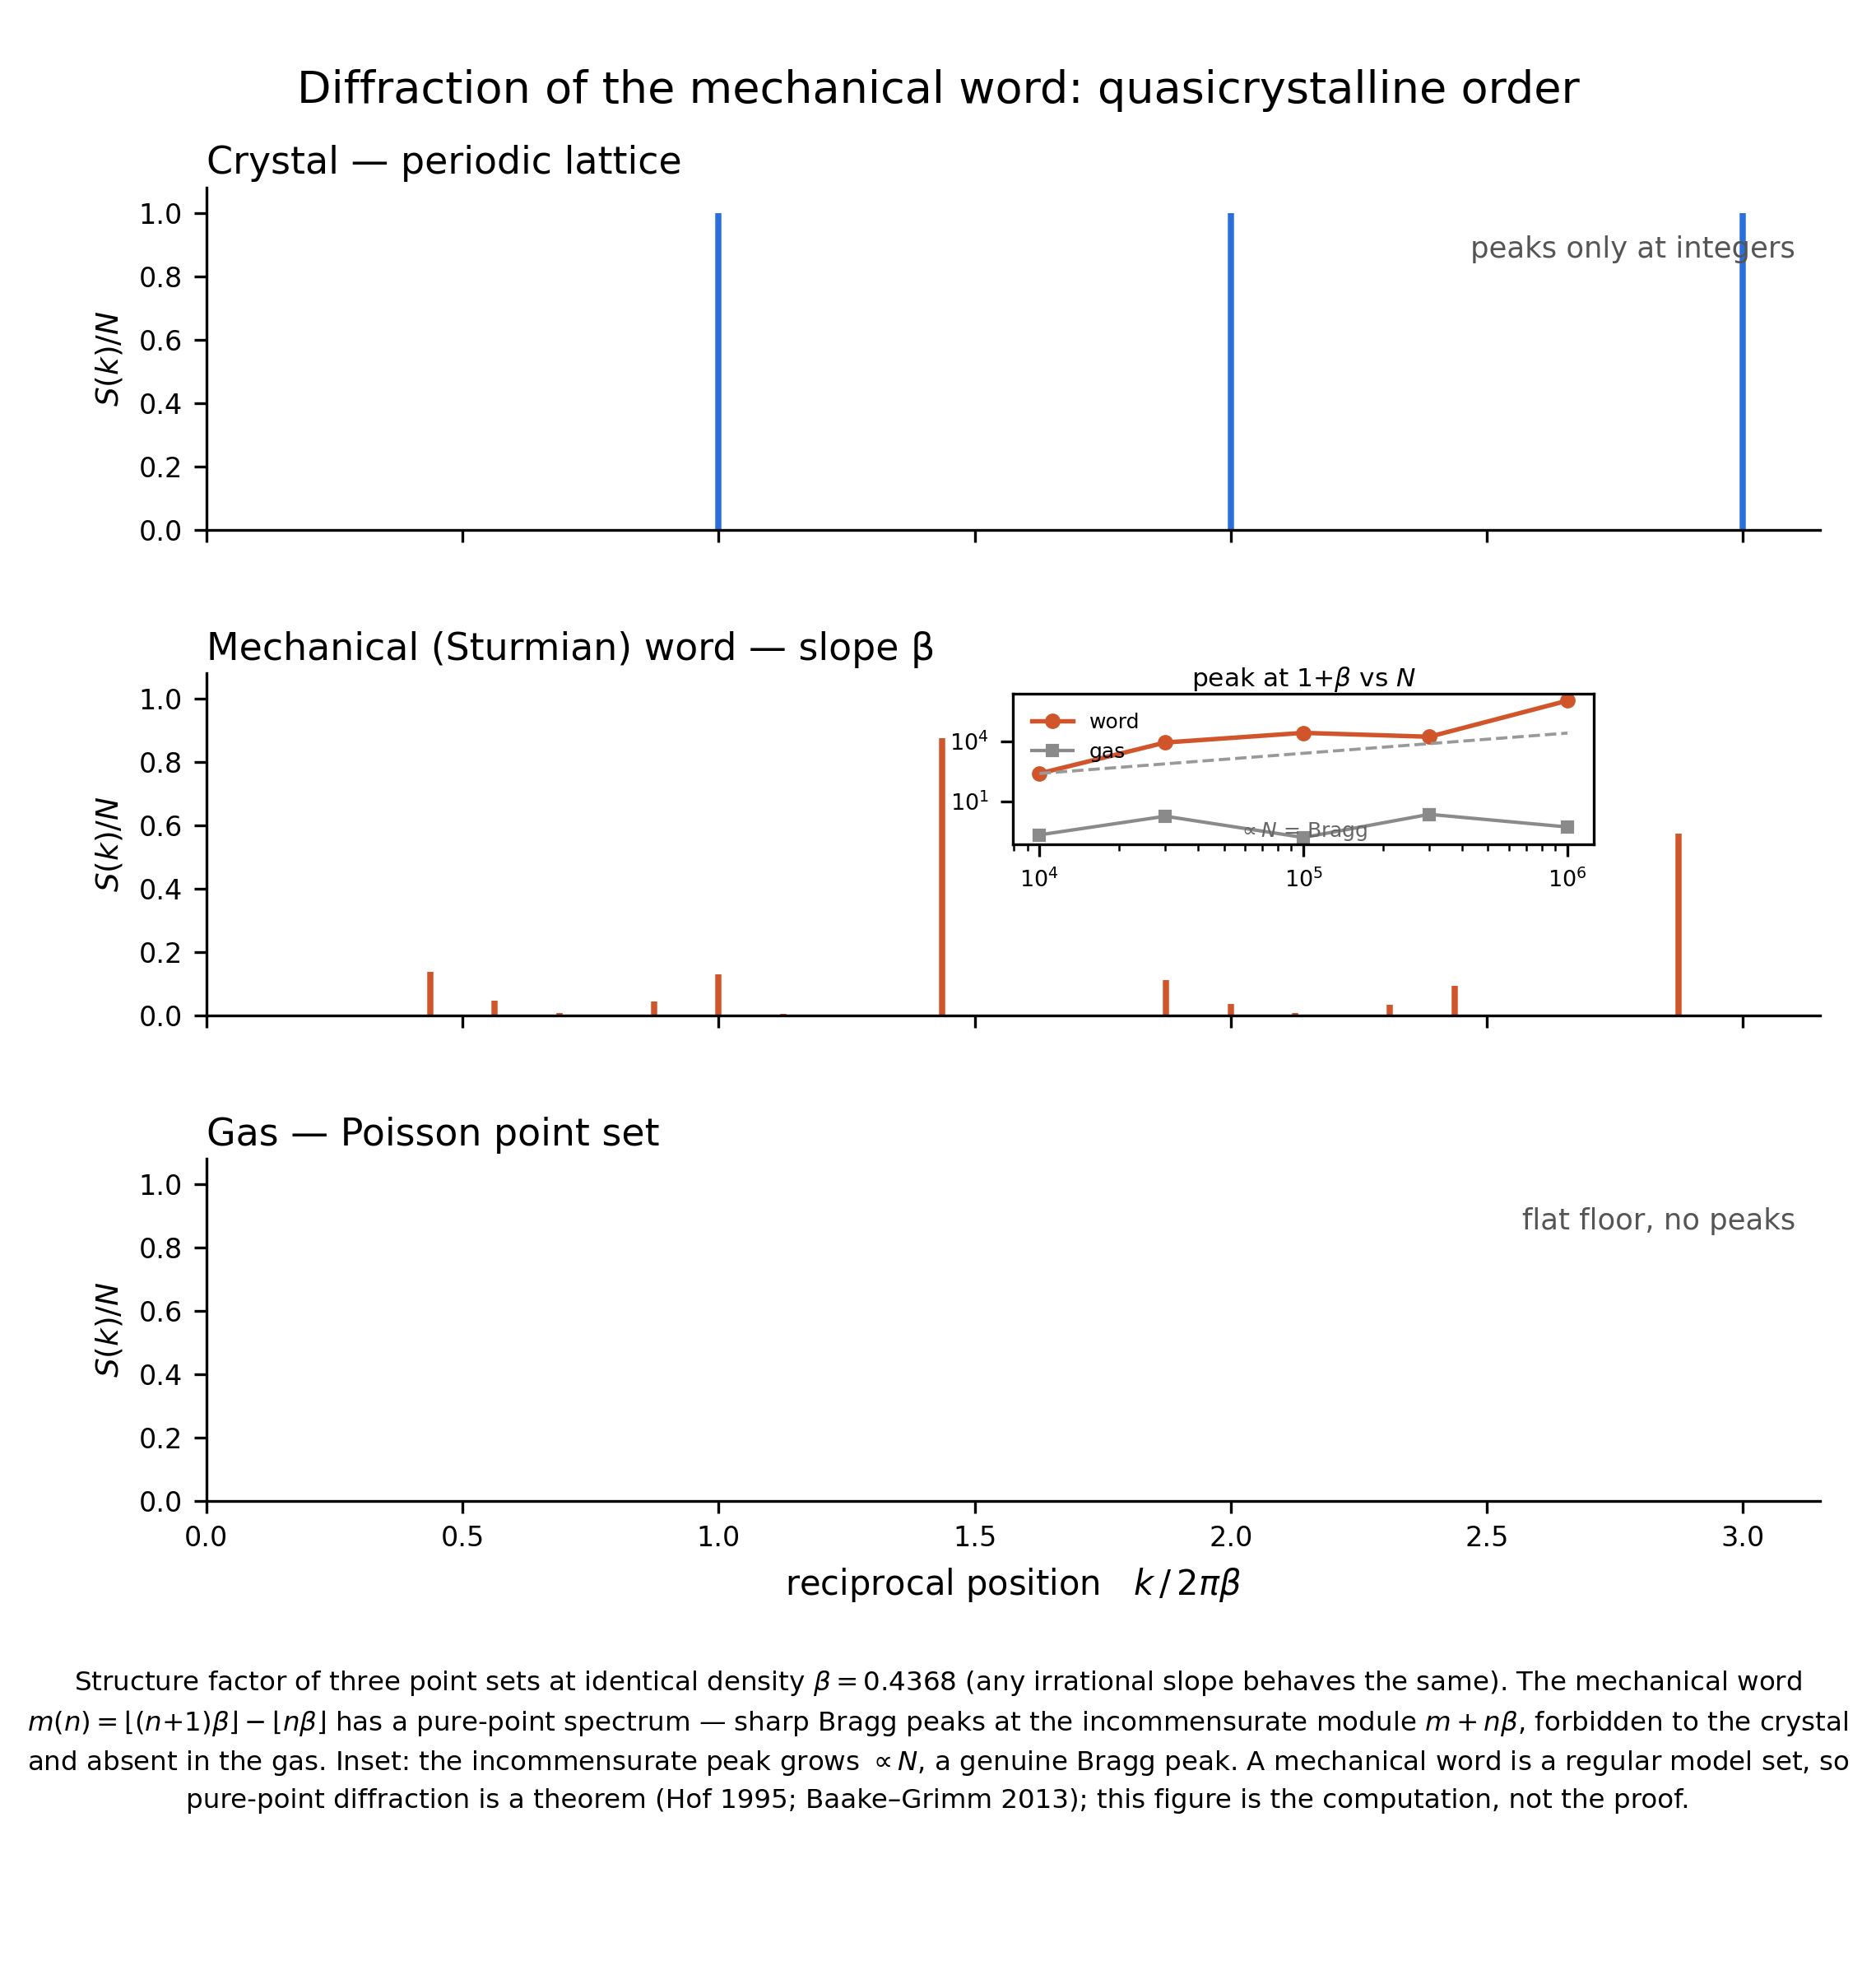
\includegraphics[width=\linewidth]{figure.png}
\caption{Diffraction of the mechanical word (computed, not proved). Structure
factor $S(k)/N$ for three point sets of identical density
$\beta = 0.4367860016$, sampled at $k = 2\pi\beta p$ with $p$ in the module
$\mathbb{Z} + \mathbb{Z}\beta$, at $N = 200000$. Top: the periodic crystal
$x_n = n/\beta$ --- peaks at integer $p$ only. Middle: the mechanical word
$m(n) = \lfloor (n+1)\beta \rfloor - \lfloor n\beta \rfloor$ laid out as
positions --- sharp peaks at incommensurate positions $m + n\beta$, forbidden
to the crystal and absent in the gas; the inset shows the intensity of the
peak at $p = 1 + \beta$ growing in proportion to $N$ (a genuine Bragg peak)
while the gas stays $O(1)$. Bottom: the Poisson set --- flat, no peaks. Every
number here is a finite-$N$ computation from the \texttt{diffraction/} folder;
the pure-point statement it illustrates is a cited theorem
\cite{hof1995, schlottmann2000, baakegrimm2013}, not a result of this paper's
formalization.}
\label{fig:diffraction}
\end{figure}

\begin{remark}[Why this must happen --- cited, not formalized]
\label{rem:modelset}
A mechanical word of irrational slope is a regular cut-and-project (model)
set: the projection to the line of the points of $\mathbb{Z}^2$ lying in a
strip of irrational slope. Regular model sets have pure-point diffraction.
This is a theorem of Hof \cite{hof1995}, extended by Schlottmann
\cite{schlottmann2000}; see Baake and Grimm \cite{baakegrimm2013} for a
systematic treatment. It is classical: it is \emph{not} formalized in the
accompanying repository, and the computation above is finite-$N$ evidence
consistent with it, not a proof of it. The figure is the computation; the
citation is the proof.
\end{remark}

Thus the kernel-verified dichotomy of Section~\ref{sec:word} --- no period for
any irrational slope (\texttt{Time.aperiodic}) yet window counts balanced to
within one (\texttt{Time.balanced}) --- is, spectrally, quasicrystalline
order: aperiodic, but pure-point diffractive.

\begin{remark}[Reproducibility]
\label{rem:repro}
In the repository, \texttt{python3 diffraction.py} prints the peak table and
the $N$-scaling above, and \texttt{python3 make\_figure.py} re-renders
Figure~\ref{fig:diffraction} (NumPy, plus Matplotlib for the figure). The run
is deterministic (seed $0$) except for the Poisson comparison set, whose flat
spectrum is seed-independent.
\end{remark}

\section{Necessity: what is forced, what is cited, what is open}
\label{sec:frontier}

The kernel-verified results of this paper are sufficiency results. Section~\ref{sec:word} proves that the word $m(n) = \lfloor (n+1)\beta \rfloor - \lfloor n\beta \rfloor$ meets all four demands set out in the introduction: it is two-valued (\texttt{Time.m\_mem}), its frequency of ones converges to $\beta$ (\texttt{Time.density\_tendsto}), it has no period when $\beta$ is irrational (\texttt{Time.aperiodic}), and any two windows of equal length carry one-counts differing by at most one (\texttt{Time.balanced}). Section~\ref{sec:boundary} proves that the two defining polynomials sit on opposite sides of the unit circle. A \emph{necessity} statement --- the four demands force this structure and no other --- requires converses, and the converses are classical theorems that we cite but have not formalized. This section states the three classical characterizations that frame the necessity question, records exactly how far the kernel-verified material reaches into each, and estimates what a formalization of the remainder would cost. Nothing in the earlier sections depends on the unformalized converses; they mark the frontier.

\subsection{The Pisot boundary}

\begin{theorem}[Pisot; classical, cited, not formalized here]
\label{thm:pisot}
Let $\theta > 1$ be a real algebraic integer. Then $\operatorname{dist}(\theta^n, \mathbb{Z}) \to 0$ as $n \to \infty$ if and only if every Galois conjugate $\theta' \neq \theta$ of $\theta$ satisfies $|\theta'| < 1$. Such $\theta$ are the Pisot numbers \cite{bertin1992}.
\end{theorem}

Section~\ref{sec:boundary} kernel-verifies the concrete instance of the conjugate condition for the two polynomials of this paper: every non-real root $z$ of $x^3 - x - 1$ satisfies $\lVert z \rVert < 1$ (\texttt{Time.cubic\_conj\_norm\_lt\_one}), every non-real root $w$ of $x^4 - x - 1$ satisfies $\lVert w \rVert > 1$ (\texttt{Time.quartic\_conj\_norm\_gt\_one}), and the conjunction is packaged as a dichotomy (\texttt{Time.pisot\_boundary\_dichotomy}). Since $x^3 - x - 1$ has exactly one real root, the non-real pair exhausts the conjugates of $\rho$, so $\rho$ meets Pisot's criterion; for $Q$, a single conjugate of modulus greater than one already disqualifies it. What is \emph{not} formalized is Theorem~\ref{thm:pisot} itself, in either direction: Mathlib v4.31.0 contains no Pisot--Vijayaraghavan theory at all --- not even the definition of a Pisot number --- so the passage from the kernel-verified conjugate positions to the settling statement $\operatorname{dist}(\rho^n, \mathbb{Z}) \to 0$ is cited, not formalized. (The forward direction for the single number $\rho$ is elementary --- the power sum $\rho^n + z^n + \bar{z}^n$ is a rational integer satisfying $t_{n+3} = t_{n+1} + t_n$, and the conjugate terms decay geometrically --- and would be a natural first extension of Section~\ref{sec:boundary}; it too is currently unformalized.)

\subsection{The Sturmian characterization}

\begin{theorem}[Morse--Hedlund; classical, cited, not formalized here]
\label{thm:morsehedlund}
A sequence $s : \mathbb{N} \to \{0,1\}$ is balanced and aperiodic if and only if there exist an irrational $\alpha \in (0,1)$ and an intercept $x$ such that $s$ is the mechanical word $s(n) = \lfloor (n+1)\alpha + x \rfloor - \lfloor n\alpha + x \rfloor$ (or its upper variant) \cite{morsehedlund1940}; see also \cite{lothaire2002}.
\end{theorem}

The forward direction is kernel-verified in Section~\ref{sec:word}, in a form slightly more general than the classical statement: balance holds for \emph{every} real slope (\texttt{Time.balanced} carries no irrationality hypothesis), and aperiodicity holds for every irrational slope, the irrationality entering as an explicit hypothesis as recorded there (\texttt{Time.aperiodic}). The converse is the necessity half --- it asserts that the four demands are satisfiable \emph{only} by mechanical words of irrational slope --- and it is not formalized. A realistic estimate for formalizing it is $1200$--$2500$ lines of Lean. The estimate is dominated by infrastructure: Mathlib today has no combinatorics on words whatsoever --- no factor sets, no subword complexity function, no balance predicate --- so every definition the converse quantifies over must be built first. On top of that, the proof needs three nontrivial lemmas:
\begin{enumerate}
\item \emph{Frequency existence.} A balanced sequence has a well-defined frequency of ones, obtained by a subadditivity argument; Fekete's lemma is available as Mathlib's \texttt{Analysis.Subadditive}, which shortens this step.
\item \emph{The rational case.} A balanced sequence whose frequency is rational is eventually periodic; hence aperiodicity forces the frequency to be irrational.
\item \emph{Intercept reconstruction.} Given a balanced aperiodic sequence of irrational frequency $\alpha$, one must exhibit the intercept $x$ realizing it as a mechanical word; the natural proof runs through equidistribution of the rotation by $\alpha$ on $\mathbb{R}/\mathbb{Z}$, where Mathlib's density theorems for \texttt{AddCircle} and its rotation-number theory give partial support.
\end{enumerate}
The low end of the estimate covers the three lemmas over a minimal interface; the high end covers a reusable combinatorics-on-words development.

\subsection{Siegel minimality}

\begin{theorem}[Siegel; classical, cited, not formalized here]
\label{thm:siegel}
The smallest Pisot number is the real root $\rho \approx 1.324718$ of $x^3 - x - 1$ \cite{siegel1944}.
\end{theorem}

This is the statement that upgrades ``$\rho$ qualifies'' to ``$\rho$ is extremal among all qualifying bases.'' It is not formalized, and it is out of reach without a prior development of general Pisot theory: Siegel's argument is not a computation on one polynomial but an argument over the entire class of Pisot numbers, via rational functions with bounded integer coefficients, so nothing like the two-polynomial reduction of Section~\ref{sec:boundary} applies. We do not attempt a line estimate.

\begin{remark}[State of the necessity chain]
\label{rem:necessity-state}
Kernel-verified: the exhibited word satisfies the four demands (Section~\ref{sec:word}), and the conjugates of the two polynomials lie on the stated sides of the unit circle (Section~\ref{sec:boundary}). Cited: the converse of Theorem~\ref{thm:morsehedlund} (the demands force a mechanical word of irrational slope), Theorem~\ref{thm:pisot} (settling is equivalent to the conjugate condition), and Theorem~\ref{thm:siegel} ($\rho$ is the least admissible base). Open, as formalizations: all three. No claim in this paper is stated above these labels.
\end{remark}

We close with the natural formalization targets, in increasing order of difficulty, offered as an invitation: each is a well-posed statement whose meaning is already fixed by the definitions of this paper.
\begin{enumerate}
\item \emph{Slope injectivity.} If $m_{\beta} = m_{\beta'}$ pointwise for $\beta, \beta' \in [0,1]$, then $\beta = \beta'$: immediate from \texttt{Time.density\_tendsto} by uniqueness of limits, a short exercise.
\item \emph{Frequency existence for balanced sequences.} Self-contained via \texttt{Analysis.Subadditive}; a few hundred lines.
\item \emph{The full Sturmian converse} (Theorem~\ref{thm:morsehedlund}). The $1200$--$2500$ line project above; it would seed a combinatorics-on-words library for Mathlib, with the complexity characterization of Sturmian sequences ($p(n) = n+1$) as a natural milestone.
\item \emph{Pisot's theorem} (Theorem~\ref{thm:pisot}). Requires conjugate embeddings and algebraic-integer machinery, parts of which Mathlib's number-field library already provides; substantial but with a marked trail.
\item \emph{Siegel minimality} (Theorem~\ref{thm:siegel}). The summit: it presupposes the previous target together with a genuine theory of Pisot numbers.
\end{enumerate}
The first two are within reach of a newcomer to Mathlib; the third would be a real contribution to the library; the last two would formalize a distinguished chapter of twentieth-century number theory. Any of them would be welcome.

\section{Formalization notes}
\label{sec:formalization}

The formal development accompanying this paper is available at
\texttt{github.com/stalex444/arithmetic-of-time} (MIT license). It targets the
toolchain \texttt{leanprover/lean4:v4.31.0} with Mathlib pinned at
\texttt{v4.31.0} (recorded in \texttt{lean-toolchain} and
\texttt{lake-manifest.json}), and \texttt{lake build} compiles the eight
project modules in full: \texttt{Irreducibility}, \texttt{FieldNorm},
\texttt{Settling}, \texttt{SettlingReplica} (an independent second
formalization of \texttt{Settling}), \texttt{ConstantChain},
\texttt{AlgebraicIntegers}, \texttt{MechanicalWord}, and
\texttt{PisotBoundary}.

The development satisfies the following audit, which is what the label
``kernel-verified'' means throughout this paper:
\begin{itemize}
\item no \texttt{sorry} anywhere in the development;
\item no \texttt{native\_decide}: every decidable fact is checked by the Lean
  kernel itself, never delegated to trusted compiled code;
\item no custom axioms: for every theorem, \texttt{\#print axioms} reports a
  subset of $\{\texttt{propext},\ \texttt{Classical.choice},\
  \texttt{Quot.sound}\}$, the standard classical foundation of Mathlib. The
  audit is reproducible declaration by declaration, e.g.\
  \texttt{\#print axioms Time.balanced}.
\end{itemize}

One design decision deserves emphasis: irrationality of the slope is never
assumed. Every statement that requires $\beta$ irrational carries
\texttt{Irrational}~$\beta$ as an explicit hypothesis (as in
\texttt{Time.aperiodic}); no axiom asserts the irrationality of any particular
real number. The formal theorems are therefore exactly as conditional as their
statements in this paper.

The single non-formal component of the repository is the
\texttt{diffraction/} folder of Section~\ref{sec:spectral}, which is clearly
marked as computation; no Lean proof depends on anything in it. Statements
labelled ``classical'' or ``cited'' --- for instance Siegel's theorem that
$\rho$ is the smallest Pisot number \cite{siegel1944}, and the pure-point
diffraction of regular model sets \cite{hof1995, schlottmann2000} --- are
literature theorems and are not formalized here.


\begin{thebibliography}{10}

\bibitem{aarts2001}
J.~Aarts, R.~Fokkink, and G.~Kruijtzer,
\emph{Morphic numbers},
Nieuw Arch. Wiskd. (5) \textbf{2} (2001), 56--58.

\bibitem{baakegrimm2013}
M.~Baake and U.~Grimm,
\emph{Aperiodic Order. Volume 1: A Mathematical Invitation},
Encyclopedia of Mathematics and its Applications \textbf{149},
Cambridge University Press, Cambridge, 2013.

\bibitem{bertin1992}
M.-J. Bertin, A.~Decomps-Guilloux, M.~Grandet-Hugot,
M.~Pathiaux-Delefosse, and J.-P. Schreiber,
\emph{Pisot and Salem Numbers},
Birkh\"auser, Basel, 1992.

\bibitem{hof1995}
A.~Hof,
\emph{On diffraction by aperiodic structures},
Comm. Math. Phys. \textbf{169} (1995), 25--43.

\bibitem{lothaire2002}
M.~Lothaire,
\emph{Algebraic Combinatorics on Words},
Encyclopedia of Mathematics and its Applications \textbf{90},
Cambridge University Press, Cambridge, 2002.

\bibitem{morsehedlund1940}
M.~Morse and G.~A. Hedlund,
\emph{Symbolic dynamics II. Sturmian trajectories},
Amer. J. Math. \textbf{62} (1940), 1--42.

\bibitem{schlottmann2000}
M.~Schlottmann,
\emph{Generalized model sets and dynamical systems},
in: Directions in Mathematical Quasicrystals
(M.~Baake and R.~V. Moody, eds.),
CRM Monograph Series \textbf{13},
Amer. Math. Soc., Providence, RI, 2000, 143--159.

\bibitem{siegel1944}
C.~L. Siegel,
\emph{Algebraic integers whose conjugates lie in the unit circle},
Duke Math. J. \textbf{11} (1944), 597--602.

\end{thebibliography}

\end{document}
